\documentclass{beamer}
\mode<presentation>
{
  \usetheme{default}
  \usecolortheme{default}
  \usefonttheme{default}
  \setbeamertemplate{navigation symbols}{}
  \setbeamertemplate{caption}[numbered]
} 

\usepackage{polski}
\usepackage[utf8]{inputenc}
\usepackage[T1]{fontenc}


\title[M2.2]{Zarządzanie Systemami Informatycznymi}
\author{Mikołaj Buczak, Karolina Woźniak}
\institute{Politechnika Śląska}
\date{\today}

\begin{document}

\begin{frame}
  \titlepage
\end{frame}

\begin{frame}{Studio IDE jako rozwiązanie wspomagające zarządzanie systemami informatycznymi }
    Studio IDE jest środowiskiem pozwalającym na tworzenie aplikacji i automatyzację tego procesu.\\
    Pozwala poświęcać więcej czasu na innowacje, a mniej na utrzymanie działania.\\
    Zwinne metodyki opracowywania i wdrażania aplikacji mogą pomóc być na bieżąco z zaległościami aplikacji.
\end{frame}
\begin{frame}{Integracja z Git}
    Studio IDE zintegrowane z Git i repozytorium aplikacji o określonym zasięgu to sposób na wdrożenie nowoczesnego, zwinnego procesu programowania w zespołach i między nimi.\\
    Korzystanie z kompatybilności z Git'em efektywnie budować aplikacje, których potrzebuje firma, spakować je oraz bezpiecznie publikować na platformie Now.
\end{frame}
\begin{frame}{Wygląd Studio IDE}
    \begin{figure}[H!]
        \centering
        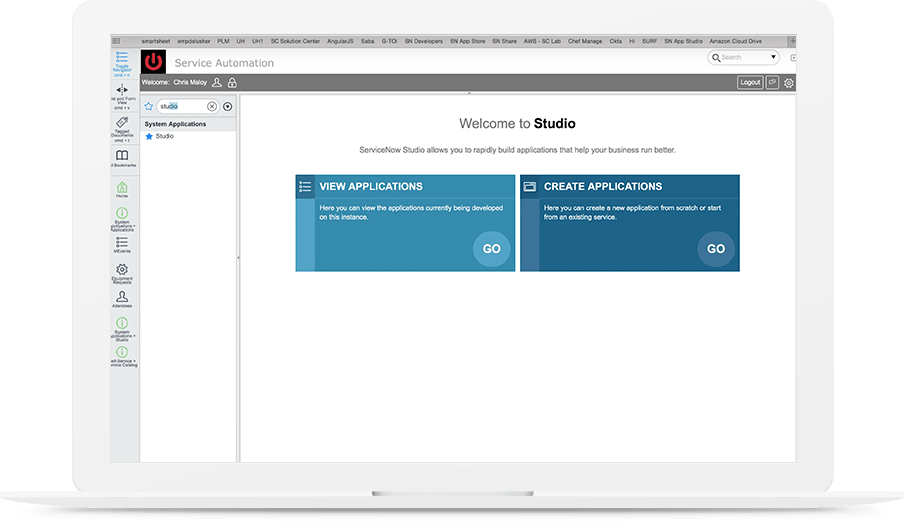
\includegraphics[width=\textwidth]{IDE.png}
        \label{fig:my_label}
    \end{figure}
\end{frame}

\begin{frame}{Tutorial}
    W kolejnych slajdach pokażemy jak przygotować instalator testowej aplikacji desktopowej w środowisku MS Windows
\end{frame}

\begin{frame}{Tutorial}
    \begin{itemize}
        \item Udostępnij swoją aplikację i utwórz plik instalatora APKA.appinstaller. Plik instalatora jest powiązany z aplikacją
        \item Udstępnij plik APKA.appinstaller. Po kliknięciu na plik otworzy powinien pokazać się interfejs instalatora aplikacji, który poprowadzi użytkownika. Od tego momentu można normalnie używać aplikacji jak każdej innej.
        \item  Gdy otrzymasz aktualizację aplikacji i chcesz udostępnić ja użytkownikom wystarczy, zaktualizować APKA.appintaller aby wskazał nową wersję aplikacji, należy również ustawić żądany typ aktualizacji. Na urządzeniach aktualizacja nastąpi automatycznie.
    \end{itemize}
\end{frame}

\begin{frame}{Discord jako alternatywa dla Slack}
    Wady:\\
    \begin{itemize}
        \item Nie pozwala dzielić wiadomości na wątki
        \item Limit wielkości przesyłanego pliku
        \item Tylko 10 podstawowych botów rozszerzających funkcjonalność
    \end{itemize}
\end{frame}
\begin{frame}{Discord jako alternatywa dla Slack}
    Zalety:\\
    \begin{itemize}
        \item Darmowy plan pozwala na więcej
        \item Konferencje wideo mogą działać w tle
        \item Nieograniczona pojemność wirtualnego dysku
        \item Funkcja Push-To-Talk
    \end{itemize}
\end{frame}

\end{document}